\section{Influenza-like-Illness Forecasting}
In this section we analyze the forecasts generated for Influenza-like-Illness
or ILI events. For ILI, we concentrated on short-term forecasts for the first 
2 years of \EMBERS. We shited our focus to long-term forecasts for the subsequent
years. We analyze both types of forecast here for general performance and 
analyze in details a few succesful forecasts which showcased the strength 
our system. There were a number of \EMBERS~ILI forecasts which significantly
deviated from the target sources. We analyzed these scenarios and discuss in 
details some of the weakness of \EMBERS. These scenarios also helped us to 
increase the robustness of our system.

\prithwi{TODO:}
\begin{itemize}
  \item Histogram of short-term forecasts QS/lead time
  \item Histogram of long-term forecasts QS/lead time
  \item CI for all categories. -- signficance of bad/good forecasts.
\end{itemize}

\subsection{successes}
\prithwi{Long-term and short term}

\begin{figure*}[tb!]
  \subcaptionbox{}{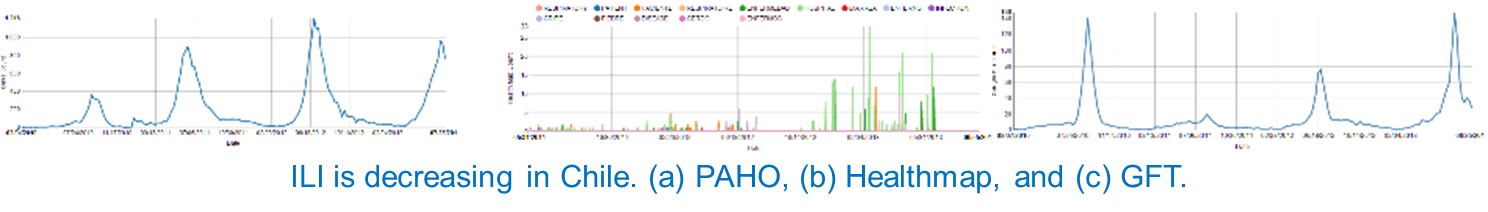
\includegraphics[width=0.9\textwidth]{../figures/ili/narrative1.png}}
  \\
  \subcaptionbox{}{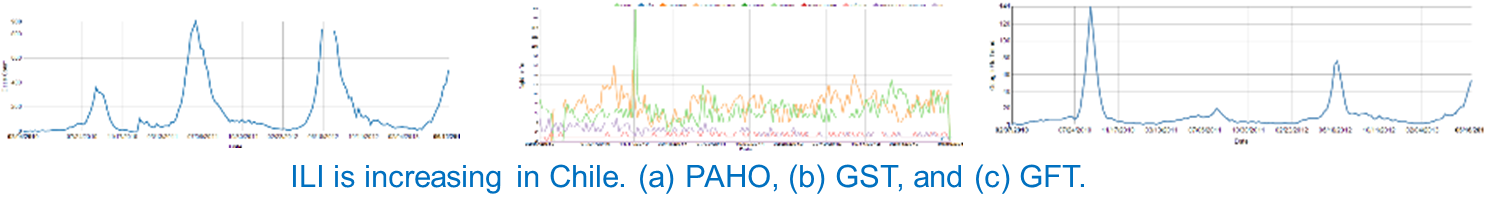
\includegraphics[width=0.9\textwidth]{../figures/ili/narrative3.png}}

  \caption{\label{} ILI short-term: success stories}
\end{figure*}

\begin{itemize}
  \item {\bf Short-term:} ILI case counts for Chile for event date 08/07/13.
    \begin{itemize}
      \item Actual value: 626
      \item First update: 581 (QS: 3.71)
      \item Second update: 619 (QS: 3.95)
      \item Possible reason: season occuring around same time, similar shape.
    \end{itemize}

  \item {\bf Long-term:} ILI seasonal predictions for Bolivia
    \begin{itemize}
      \item Total flu/SRV count
      \item Peak date for flu/SRV
    \end{itemize}
\end{itemize}

\subsection{failures}

\begin{itemize}
  \item {\bf Short-term:} ILI case counts for Argentina
    \begin{itemize}
      \item Seasonality?
    \end{itemize}
  \item {\bf Long-term:} ILI seaonal predictions for Mexico
    \begin{itemize}
      \item Shifts in seasons. 
    \end{itemize}
\end{itemize}

